\documentclass[convert={density=200}]{standalone}
\usepackage{tikz} 
\usetikzlibrary{arrows}

\begin{document}

 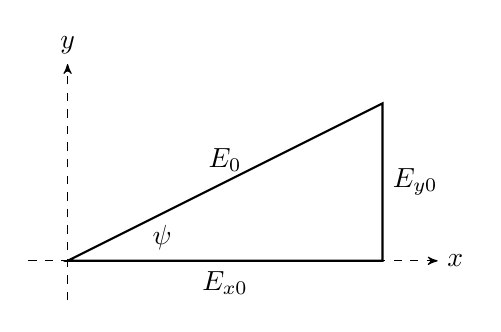
\begin{tikzpicture} [axis/.style={dashed, ->, >=stealth'}, 
 			      line/.style={thick},
 			      pile/.style={thick, ->, >=stealth', shorten <=2pt, shorten >=2pt}]
    \draw[line] 
    	    (0,0)
	-- (4,0) node[midway,below] {$E_{x0}$}
	-- (4,2) node[midway,right] {$E_{y0}$}
	-- cycle node[midway,above] {$E_0$};
    \draw[axis] (-0.5,0) -- (4.7,0) node(xline)[right] {$x$};
    \draw[axis] (0,-0.5) -- (0,2.5) node(xline)[above] {$y$};
    \node[] at (1.2,0.3) {$\psi$};
   % \draw[pile] (0,0) -- (1,2);

\end{tikzpicture}

\end{document}